\hfill \break
\hfill \break
\hfill \break
\hfill \break
\hfill \break
\hfill \break
\hfill \break
\hfill \break
\hfill \break
\hfill \break

\subsection*{Algoritmo Merge}
    El algoritmo utilizado para la realización de esta práctica es en unos aspectos muy particulares diferentes al mostrado en clase. El código que se implementa como muestra utiliza un ciclo \textit{for} para realizar el ordenamiento de los 2 subarreglos obtenidos, más esta implementación ignora el tamaño de estos subarreglos, provocando que en las verificaciones del tamaño del valor de estos se utiliza un índice fuera de los límites, genrando una excepción. \\
    
    Para subsanar este inconveniente, se utiliza en cambio, un ciclo \textit{while} que iterará las variables que recorren los 2 subarreglos hasta que una de estas al menos, exceda el límite de los índices. \\
    
    Cuando se cumpla esta condición, existe la posibilidad de que alguna de las variables no alcancé el índice máximo, significando que no se ha recorrido por completo el subarreglo. Dado que es seguro que los valores restantes sin verificar en el subarreglo restante son los mayores, se procede únicamente mediante un ciclo \textit{while} que agote los valores recorridos y los vaya ingresando en el arreglo de retorno. \\
    
    El pseudocódigo de la implementación programada se muestra en la figura \ref{PseudocodigoMerge}:

    \begin{figure}[h!]
        \centering
        \begin{verbatim}
            int[] Merge(A[],p,q,r)
                n1 = q-p+1
                n2 = r-q
                
                # Creación e inicialización de los subarreglos
                L = new int[n1]
                R = new int[n2]
                for i=0 to i<n1 do
                    L[i] = A[p+i]
                for j=0 to j<n2 do
                    R[j] = A[q+j+1]
                
                # Inicia el ordenamiento de los valores en el arreglo de entrada A
                i = 0
                j = 0
                k = p
                while i<n1 and j<n2 do
                    if L[i] <= R[j]
                        A[k] = L[i]
                        i++
                    else
                        A[k] = R[j]
                        j++
                        
                # Se terminan de ingresar los valores de los subarreglos sin recorrer completamente   
                while i<n1 do
                    A[k] = L[i]
                    i++
                    k++
                while j<n2 do
                    A[k] = R[j]
                    j++
                    k++
                    
                return A
        \end{verbatim}
        \caption{Pseudocódigo del algoritmo Merge}
        \label{PseudocodigoMerge}
    \end{figure}
    
    \newpage
    
\hfill \break
\hfill \break
\hfill \break
\hfill \break

    \subsubsection*{Complejidad de \textbf{Merge} mediante gráficas}
        Para la obtención de los pares ordenados que se grafícaron, se realizó una evaluación del número de operaciones realizadas en el algoritmo para completar su flujo. Se utilizaron arreglos generados aleatoriamente con valores entre el 0 y el 9, y según las necesidades del algoritmo, se encuentran ordenados en 2 subarreglos. \\
        
        Se varía el tamaño del arreglo con la intención de obtener los valores que se graficarán. Estos valores se tomaron de 10 en 10, empezando desde el 1 y terminando en el 200, los puntos obtenidos se muestrán en la figura \ref{PuntosMerge}.\\
        
        \begin{figure}[h!]
            \centering
            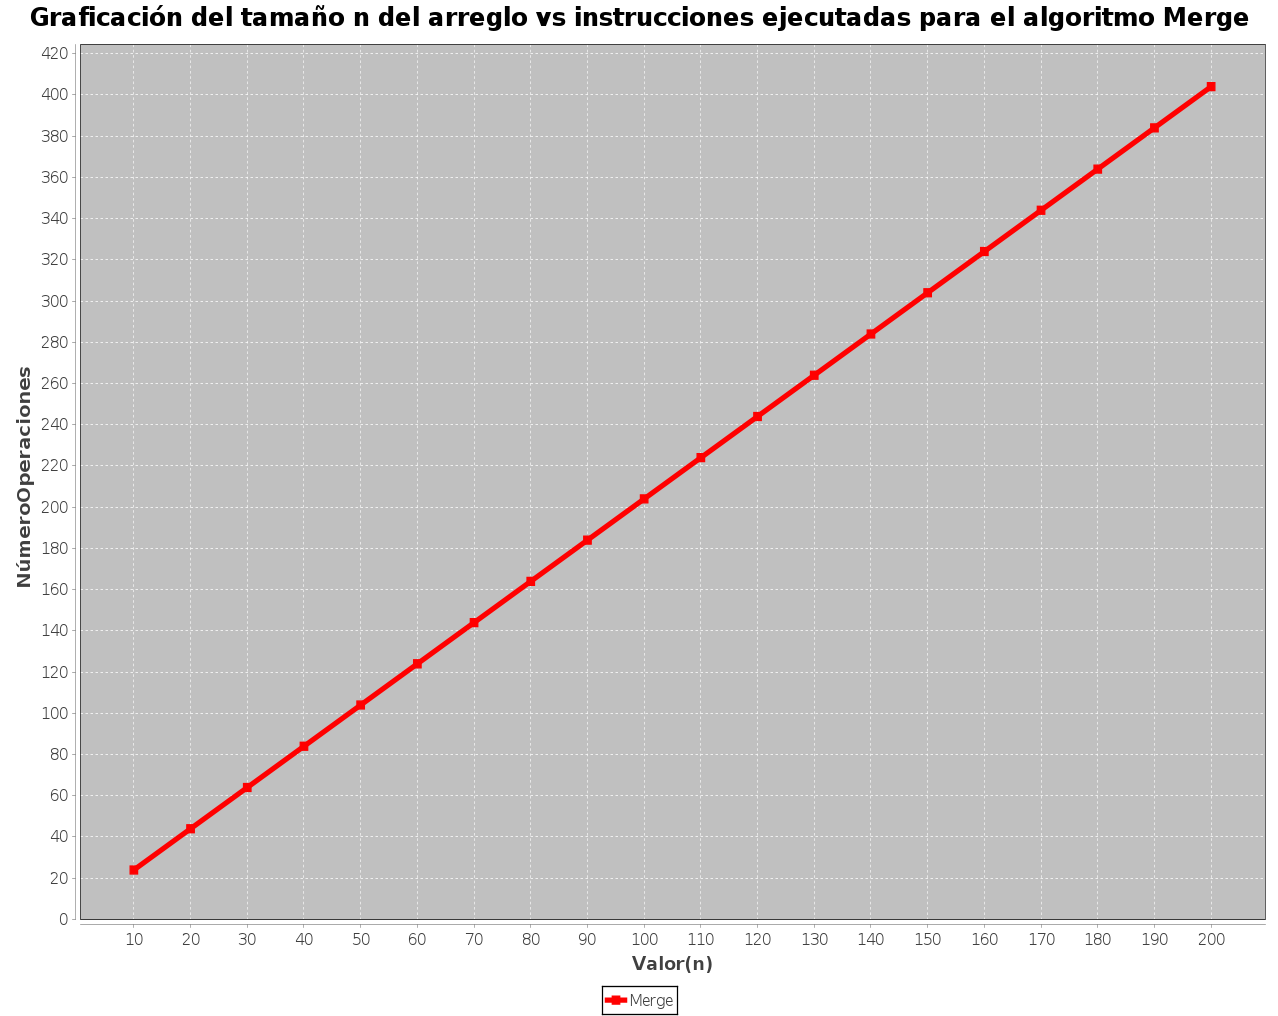
\includegraphics[width=19cm]{MergeSort/GraficaMerge.png}
            \caption{Representación gráfica de la complejidad del algoritmo Merge mediante la evaluación del número de instrucciones realizadas}
            \label{GraficaMerge}
        \end{figure}
        
        \begin{figure}[h!]
            \centering
            \begin{tabular}{c c}
            P0( 1,6 ) & \\
                P1( 10,24 ) & P11( 110,224 )\\
                P2( 20,44 ) & P12( 120,244 )\\
                P3( 30,64 ) & P13( 130,264 )\\
                P4( 40,84 ) & P14( 140,284 )\\
                P5( 50,104 ) & P15( 150,304 )\\
                P6( 60,124 ) & P16( 160,324 )\\
                P7( 70,144 ) & P17( 170,344 )\\
                P8( 80,164 ) & P18( 180,364 )\\
                P9( 90,184 ) & P19( 190,384 )\\
                P10( 100,204 ) & P20( 200,404 )\\
            \end{tabular}
            \caption{Pares ordenados obtenidos de la evaluación del algoritmo Merge}
            \label{PuntosMerge}
        \end{figure}
    
    Y la gráfica generada por estos pares se muestra en la figura \ref{GraficaMerge}.\\
    
    Se aprecia claramente en la gráfica una recta, implicando que la complejidad del algoritmo es lineal. A continuación se demuestra su relación con una ecuación lineal.\\
    
\hfill \break
\hfill \break
\hfill \break
\hfill \break

    La ecuación para la recta en su forma punto-pendiente es: \textbf{y=mx+b}
    Primero encontramos el término independiente, este término implica en el código operaciones de complejidad lineal, tales como asignaciones de variables.\\
    
    Tomaremos por facilidad, los puntos \textbf{P1} y \textbf{P2}:\\
    \begin{equation*}
        \begin{split}
            P1 \rightarrow 24= & 10m + b \\
            P2 \rightarrow 44= & 20m + b
        \end{split}
    \end{equation*}
    Se despeja la pendiente e igualan los términos:\\
    \begin{equation*}
        \begin{split}
            m= & \frac{24-b}{10} \\
            m= & \frac{44-b}{20} \\
            \\
            \frac{24-b}{10}= & \frac{44-b}{20}\\
            480-20b= & 440-10b\\
            40= & 10b\\
            b= & 4
        \end{split}
    \end{equation*}
    Ahora simplemente sustituimos el valor del término independiente en alguna de las 2 ecuaciones con la pendiente despejada:
    \begin{equation*}
        \begin{split}
            m=& \frac{24-4}{10}\\
            m=& \frac{20}{10}\\
            m=& 2
        \end{split}
    \end{equation*}
    Concluimos que los valores para el término independiente y la pendiente son:
    \begin{equation*}
        \begin{split}
            \textbf{m=} & \textbf{2}\\
            \textbf{b=} & \textbf{4}
        \end{split}
    \end{equation*}
    
    Obtenidos estos valores es fácil realizar la subsitución en la ecuación \ref{EcuacionLinealMerge} para comprobar que cualquier valor dado como tamaño \textbf{n}(correspondiente a \textbf{x}) nos dará un número de operaciones(correspondiente a \textbf{y}).
    \begin{figure}[h!]
        \centering
        \begin{equation*}
           \textbf{y=2x + 4}
        \end{equation*}
        \caption{Ecuación para el cálculo del número de operaciones realizadas en el algoritmo Merge para un tamaño \textbf{x} dado}
        \label{EcuacionLinealMerge}
    \end{figure}
    
    Se concluye entonces que:
    \begin{equation*}
        Merge(n) \in \Theta(n)
    \end{equation*}
    \newpage
    
    
    
    
    
    
    
    \subsubsection*{Complejidad de \textbf{Merge} analíticamente}
    
    Ahora nos apoyamos en el pseudocódigo \ref{PseudocodigoMerge} para el análisis por bloque de las instrucciones en la función Merge: \\
    
    El primer bloque analizado corresponde solamente a asignaciones, correspondiendoles una complejidad constante:
    \begin{equation*}
        \left.
            \begin{aligned}
                \text{n1 = q-p+1} \\
                \text{n = r-q} \\
                \text{L = new int[n1]} \\
                \text{R = new int[n2]}
            \end{aligned}
        \right\}
        \quad\Theta(1)
    \end{equation*}
    
    El siguiente bloque de instrucciones dan los valores a los subarreglos que deben de combinarse para integrarse en 1 solo ordenado:
    \begin{equation*}
        \left.
            \begin{aligned}
                \text{for i=0 to i}<\text{n1 do} \\
                \text{L[i] = A[p+1]} \\
                \text{for j=0 to j}<\text{n2 do}\\
                \text{R[j] = A[q+j+1]}
            \end{aligned}
        \right\}
        \quad\Theta(n)
    \end{equation*}
    
    Le sigue un bloque con asignaciones que son importantes para el correcto ordenamiento de los arreglos.
    La variable \textbf{i} representa el índice del subarreglo \textbf{L}.
    La variable \textbf{j} representa el índice del subarreglo \textbf{R}.
    La variable \textbf{k} representa el índice del arreglo origen \textbf{A}, y por lo tanto donde se realizarán las inserciones de valores ordenadamente. Esta variable se inicia en el valor de \textbf{p}, que es la posición del primer elemento que se ordena y por lo tanto también es la posición del primer elemento del subarreglo \textbf{L}:
    \begin{equation*}
        \left.
            \begin{aligned}
                \text{i = 0} \\
                \text{j = 0} \\
                \text{k = p}
            \end{aligned}
        \right\}
        \quad\Theta(1)
    \end{equation*}
    
    Inicia el ordenamiento de los valores que contiene \textbf{A} mediante la evaluación de los contenidos en los subarreglos:
    \begin{equation*}
        \left.
            \begin{aligned}
                \left.
                    \begin{aligned}
                        \text{while i}<\text{n1 and j}<\text{n2 do} \\
                        \text{if L[i] <= R[j]} \\
                        \text{A[k] = L[i]} \\
                        \text{i++} \\
                        \text{else} \\
                        \text{A[k] = R[j]} \\
                        \text{j++} \\
                    \end{aligned}
                \right\}
                \quad\Theta(n1+n2-c)
                \\
                \left.
                    \begin{aligned}
                        \left.
                            \begin{aligned}
                                \text{while i}<\text{n1 do}\\
                                \text{A[k] = L[i]}\\
                                \text{i++} \\
                                \text{k++}
                            \end{aligned}
                        \right\}
                        \quad \Theta(c_1)
                        \\
                        \left.
                            \begin{aligned}
                                \text{while i}<\text{n1 do}\\
                                \text{A[k] = R[j]}\\
                                \text{j++} \\
                                \text{k++}
                            \end{aligned}
                        \right\}
                        \quad \Theta(c_2)
                    \end{aligned}
                \right\}
                \quad\Theta(c)
            \end{aligned}
        \right\}
        \quad\Theta(n)
    \end{equation*}
    En el primer bloque observamos una complejidad \textbf{n1+n2-c}, esto implica que se recorren los subarreglos \textbf{L} y \textbf{R} hasta que se alcance el límite de uno de ellos, por esta razón se agrega una \textbf{c} constate que indica la diferencia de índices restantes para el subarreglo que aún no se ha agotado hasta el límite de sus valores.\\
    
    Por esta misma razón, los siguientes 2 bloques iterarán aumentando el valor de los índices de los 2 subarreglos hasta que los 2 ingresen todos los valores en A. Siempre se dará el caso donde solo 1 de estos \textit{while} iterará, mientras el otro solo realiza la verificación pero no ejecuta su interior. Las 2 constantes(\textbf{c1,c2}) pueden tomar el valor de 0 o \textbf{c}, resultandonos al realizar la suma de sus complejidades tan solo la constante \textbf{c}.\\
    
    Finalmente la complejidad de estos 3 bloques nos resulta: $n1+n2-c+c = n1+n2$
    Pero el valor de esta suma es igual al tamaño del arreglo \textbf{A} original, por lo que se concluye que el valor de ese bloque es lineal.\\
    
    La suma de las complejidades de los bloques nos queda de la siguiente manera:
    \begin{equation*}
        \Theta(1) + \Theta(n) + \Theta(1) + \Theta(n) = 2\Theta(n) + 2\Theta(1) = 2\Theta(n)
    \end{equation*}
    El 2 que multiplica a la complejidad lineal, es la constante encontrada en el análisis \textit{a posteriori} realizada en la sección anterior, sin embargo esta cifra nos es solamente útil si deseamos expresar una ecuación que acote de forma justa a la resultada por este algoritmo, no siendo el caso presente se concluye que:
    \begin{equation*}
        Merge(n) \in \Theta(n)
    \end{equation*}
    
    
    
    
\subsection*{Algoritmo MergeSort}
    Para la implementación de este algoritmo se utilizó el mismo código mostrado en el video. Contiene pocas líneas de código y es bastante claro en su funcionamiento, pero es gracias a la utilización del algoritmo \textbf{Merge} que este funciona enteramente como divisor de subproblemas, y que mediante \textbf{Merge} se irán uniendo para integrar y obtener el ordenamiento de todo el arreglo. \\
    
    El pseudocódigo de este se muestra en la siguiente figura \ref{CodigoMergeSort}:
    \begin{figure}[!h]
        \centering
        \begin{verbatim}
            int[] MergeSort(A[],p,r)
                if p<r
                    q = (p+r)/2
                    
                    MergeSort(A,p,q)
                    MergeSort(A,q+1,r)
                    Merge(A,p,q,r)
                    
                    return A
        \end{verbatim}
        \caption{Pseudocódigo del algoritmo MergeSort}
        \label{PseudocodigoMergeSort}
    \end{figure}
    
    \subsubsection*{Complejidad de \textbf{MergeSort} mediante gráficas}
    
    Para la obtención de los pares ordenados que se grafícaron, se realizó una evaluación del número de operaciones realizadas en el algoritmo para completar su flujo. Se utilizaron arreglos generados aleatoriamente con valores entre el 0 y el 9.
        
        Se varía el tamaño del arreglo con la intención de obtener los valores que se graficarán. Estos valores se tomaron de 10 en 10, empezando en el 1 y terminando en el 200, los puntos obtenidos se muestrán en la figura \ref{PuntosMergeSort}.\\
        
        \begin{figure}[h!]
            \centering
            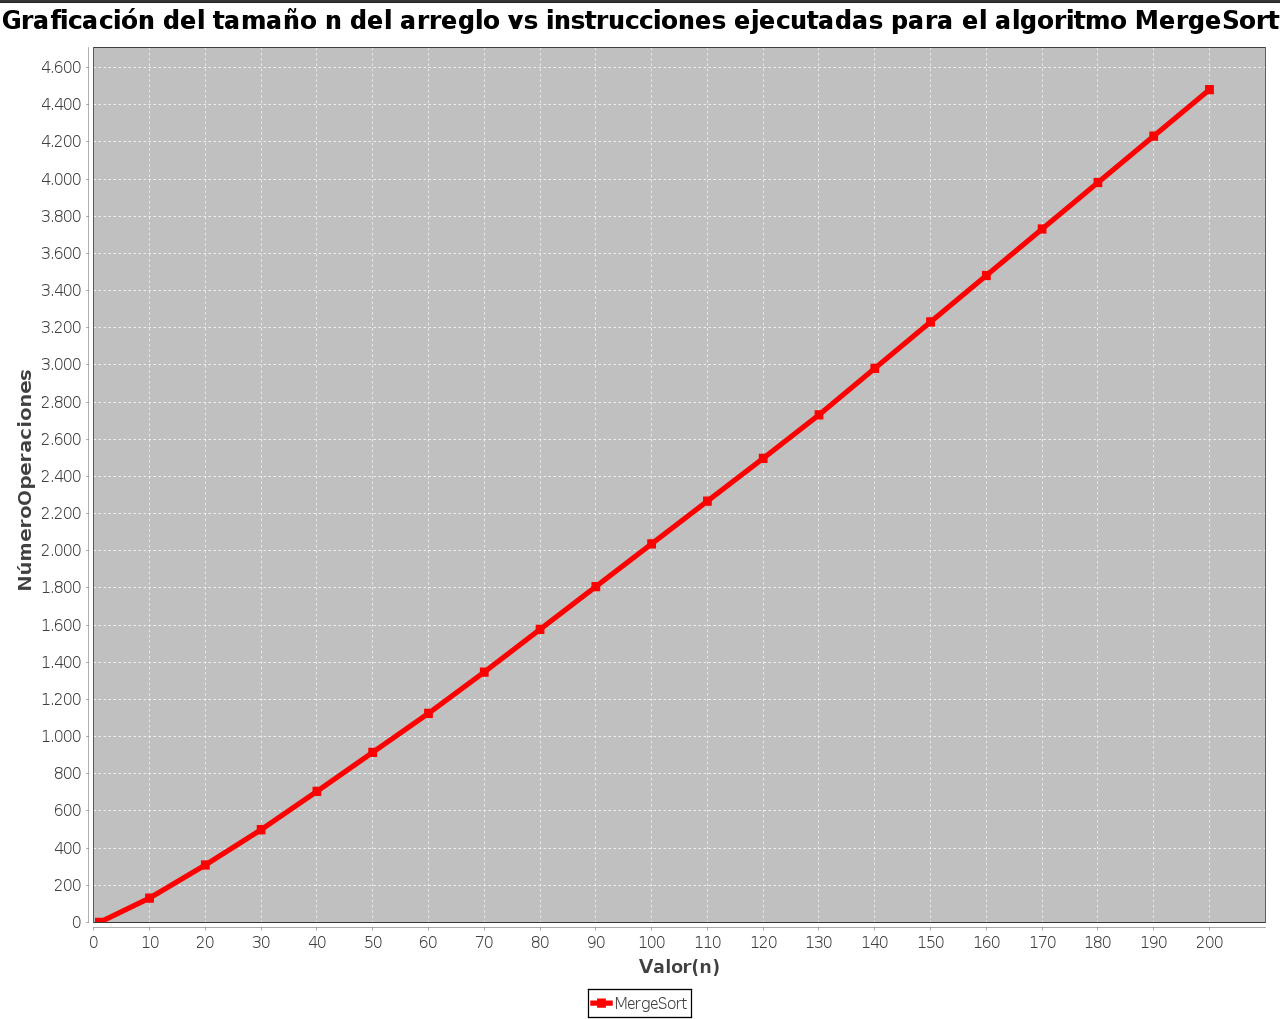
\includegraphics[width=17cm]{MergeSort/GraficaMergeSort.png}
            \caption{Representación gráfica de la complejidad del algoritmo MergeSort mediante la evaluación del número de instrucciones realizadas}
            \label{GraficaMergeSort}
        \end{figure}
        
        \begin{figure}[h!]
            \centering
            \begin{tabular}{c c}
                P0( 1, 0 ) & \\
                P1( 10,131 ) & P11( 110,2267 )\\
                P2( 20,309 ) & P12( 120,2497 )\\
                P3( 30,499 ) & P13( 130,2731 )\\
                P4( 40,705 ) & P14( 140,2981 )\\
                P5( 50,915 ) & P15( 150,3231 )\\
                P6( 60,1125 ) & P16( 160,3481 )\\
                P7( 70,1347 ) & P17( 170,3731 )\\
                P8( 80,1577 ) & P18( 180,3981 )\\
                P9( 90,1807 ) & P19( 190,4231 )\\
                P10( 100,2037 ) & P20( 200,4481 )\\
            \end{tabular}
            \caption{Pares ordenados obtenidos de la evaluación del algoritmo Merge}
            \label{PuntosMergeSort}
        \end{figure}
    
    Y la gráfica generada por estos pares se muestra en la figura \ref{GraficaMerge}.\\
    
    Aparentemente, dado el primer vistazo pareciera ser una gráfica generada por la ecuación de una recta, pero se tiene una particularidad en el \textbf{P0}, donde para el valor de la unidad en el tamaño del arreglo, y en el caso del análisis que sería para el valor de la \textbf{x}, se obtiene el valor 0. Si se evaluara tal valor en la ecuación \textbf{y=mx+b}, obtendríamos un valor definitivamente mayor a 0. \\
    
    Debido a esto podemos descartar una complejidad lineal para el algoritmo, pues no existe un valor para la pendiente \textbf{m} y para la constante \textbf{b} que al sustituir nos describa los puntos obtenidos. Así entonces y considerando según la jerarquía de cotas una superior a la complejidad lineal. \\
    
    La cota mayor inmediata es el \textbf{nlogn}, tal que ahora se muestran gráficas en la figura \ref{GraficasPropuestaMergeSort}, que comparan el comportamiento de la obtenido por el algoritmo y las 2 ecuaciones consideradas hasta el momento:\\
    
    \begin{figure}[h!]
        \centering
        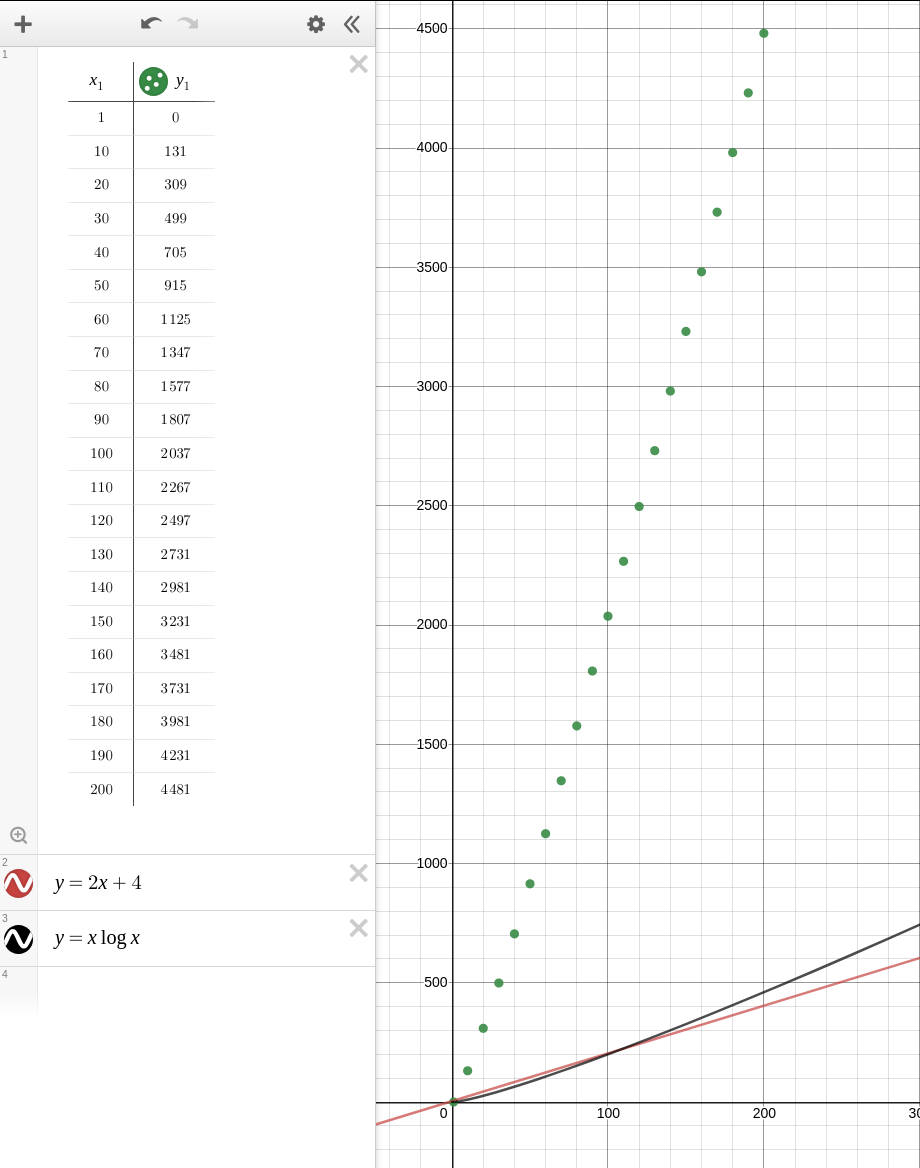
\includegraphics[width=15cm]{MergeSort/GraficasPropuestaMergeSort.png}
        \caption{Los puntos verdes corresponden a los obtenidos en la evaluación del algoritmo.\\ La gráfica en color rojo corresponde a la ecuación que describe la complejidad obtenido para el algoritmo \textbf{Merge}.\\ La gráfica en color negro corresponde a la cota propuesta para la complejidad de \textbf{MergeSort}}
        \label{GraficasPropuestaMergeSort}
    \end{figure}
    
    \hfill \break
    \hfill \break
    \hfill \break
    \hfill \break
    \hfill \break
    
    Hasta este momento en la figura \ref{GraficasPropuestaMergeSort} tan solo es visible que ciertamente la ecuación \textbf{xlogx} tiende a crecer más rápidamente que la ecuación lineal a partir de un valor de \textbf{x}, pero evidentemente esta ecuación crece mucho más lento que lo que hace la obtenida por nuestro análisis del algoritmo. Para acortar esta brecha entre las 2, se propone entonces agregar una constante que multiplique a la ecuación tal como lo muestra la figura \ref{GraficasFinalesMergeSort}.
    
    \begin{figure}[h!]
        \centering
        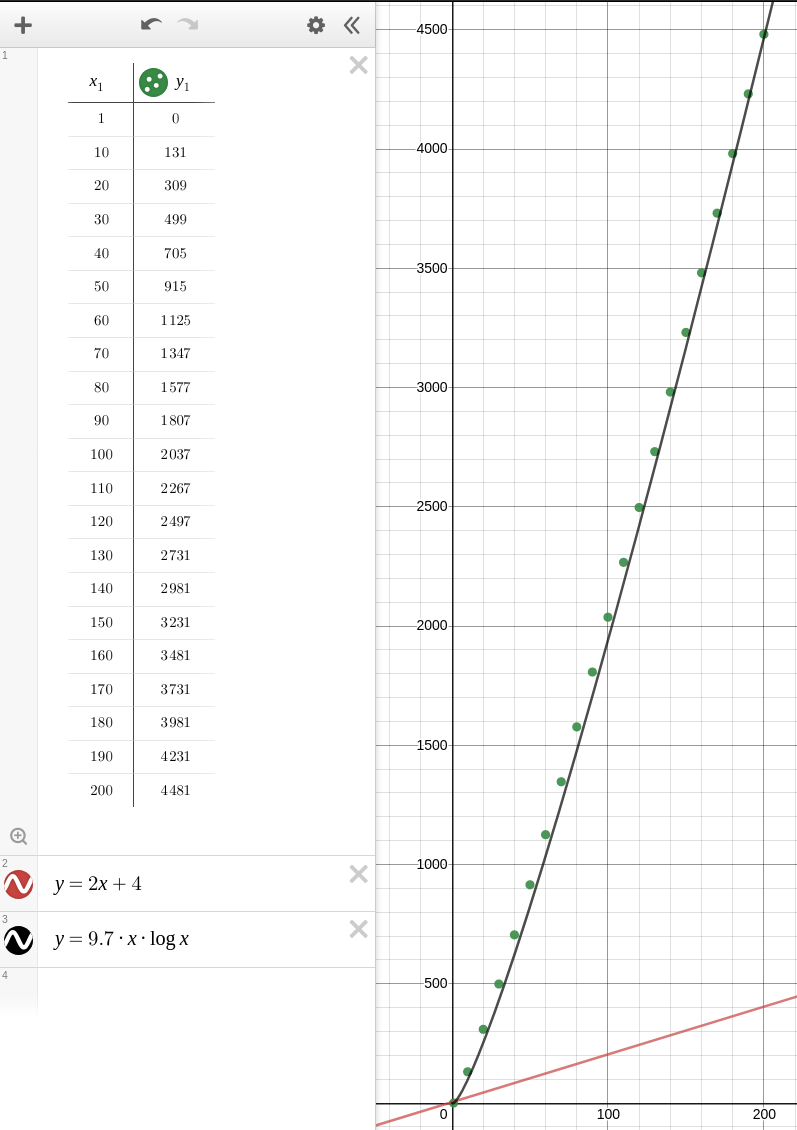
\includegraphics[width=13cm]{MergeSort/GraficasFinalesMergeSort.png}
        \caption{Los puntos verdes corresponden a los obtenidos en la evaluación del algoritmo.\\ La gráfica en color rojo corresponde a la ecuación que describe la complejidad obtenido para el algoritmo \textbf{Merge}.\\ La gráfica en color negro corresponde a la cota propuesta para la complejidad de \textbf{MergeSort}}
        \label{GraficasFinalesMergeSort}
    \end{figure}
    \newpage
    
    La asignación de la constante multiplicativa fue asignada de forma arbritaria a la que más justamente se acomodaba a la trayectoria de los puntos, esto con el único fin de mostrar que existe una posible \textbf{c} constante que multiplique a la ecuación para describir exactamente al comportamiento del algoritmo, y de esta forma nos es posible concluir que la complejidad del algoritmo \textbf{MergeSort} es:
    \begin{equation*}
        \text{MergeSort} \in \Theta(nlogn)
    \end{equation*}
    
    \newpage
    
    \subsubsection*{Complejidad de \textbf{MergeSort} analíticamente}
        Retomamos la figura \ref{PseudocodigoMergeSort} que contiene el pseudocódigo de la función, y se inicia el análisis por bloques de la función:
    \begin{equation*}
        \left.
            \begin{aligned}
                \bigl.
                    \text{if p}<r
                \bigr\}
                \quad\Theta(1)
                \\
                \bigl.
                    \text{q = (p+r)/2}
                \bigr\}
                \quad\Theta(1)
                \\
                \bigl.
                    \text{MergeSort(A,p,q)}
                \bigr\}
                \quad\text{M}\left(\frac{n}{2}\right)
                \\
                \bigl.
                    \text{MergeSort(A,q+1,r)}
                \bigr\}
                \quad\text{M}\left(\frac{n}{2}\right)
                \\
                \bigl.
                    \text{Merge(A,p,q,r)}
                \bigr\}
                \quad\Theta(n)
            \end{aligned}
        \right\}
        \quad2\text{M}\left(\frac{n}{2}\right)+\Theta(n)
    \end{equation*}
    
    De donde vamos a considerar a \textbf{M(n)} como la ecuación de recursividad en \ref{EcuacionRecursivaMergeSort}:
    \begin{figure}[h!]
        \centering
        \begin{equation*}
            M(n)=2M \left( \frac{n}{2} \right) +\Theta(n)
        \end{equation*}
        \caption{Ecuación de recursividad para el algoritmo MergeSort}
        \label{EcuacionRecursivaMergeSort}
    \end{figure}
    
    De la ecuación se idenfican:\\
    $a = 2$\\
    $b = 2$\\
    $f(n) = cn$
    
    Con los elementos identificados de la ecuación, evaluamos para obtener la complejidad usando el \textit{Método maestro}.\\
    Como primer paso obtenemos los valores de la siguiente ecuación:
    \begin{equation*}
        n^{log_ba} = n^{log2} = n
    \end{equation*}
    
    Y verificamos con respecto a \textbf{f(n)}:
    \begin{equation*}
        n = n^{log_ba} = f(n) = n
    \end{equation*}
    
    Dado que esto se cumple, obtenemos la complejidad mediante el caso \textbf{II} del Teorema maestro:
    \begin{equation*}
        M(n) \in \Theta(n^{log_ba}logn) \Rightarrow M(n) \in \Theta(nlogn)
    \end{equation*}
